% flashcards-title: Tenths on a centimeter scale
% flashcards-desc: A scale from four to five centimeters has ten equal divisions and marks A at the seventh division after four.
\documentclass[dvisvgm,tikz,border=8pt]{standalone}\usetikzlibrary{arrows.meta,patterns}

\definecolor{qraNavy}{HTML}{17324D}
\definecolor{qraBlue}{HTML}{2B6CB0}
\definecolor{qraGold}{HTML}{B7791F}
\definecolor{qraPale}{HTML}{EAF2F8}
\definecolor{qraGray}{HTML}{5C6773}

\tikzset{
  qra axis/.style={draw=qraNavy, line width=1.2pt},
  qra tick/.style={draw=qraNavy, line width=1pt},
  qra guide/.style={draw=qraGray, densely dashed, line width=0.8pt},
  qra counter/.style={circle, draw=qraNavy, fill=qraPale, line width=0.9pt, minimum size=7mm, inner sep=0pt},
  qra label/.style={font=\sffamily\bfseries, text=qraNavy},
  qra small label/.style={font=\sffamily, text=qraNavy},
}

\begin{document}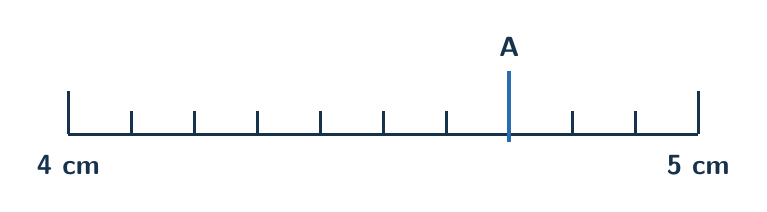
\begin{tikzpicture}[x=.8cm,y=1cm]\draw[qra axis](0,0)--(10,0);\foreach \x in {0,...,10}{\draw[qra tick](\x,0)--(\x,{ifthenelse(mod(\x,10)==0,.55,.3)});}\node[qra label,below=4pt]at(0,0){4 cm};\node[qra label,below=4pt]at(10,0){5 cm};\draw[qraBlue,line width=1.4pt](7,-.1)--(7,.8);\node[qra label,above=2pt]at(7,.8){A};\end{tikzpicture}\end{document}
